\documentclass[spanish,a4paper,12pt,oneside]{extreport}

\usepackage[dvips]{graphicx}
\usepackage[dvips]{epsfig}
\usepackage[utf8]{inputenc}
\usepackage[spanish]{babel}
\usepackage{alltt}

\usepackage[ruled,vlined,commentsnumbered,linesnumbered,inoutnumbered,titlenotnumbered,noend]{algorithm2e}
\SetKwRepeat{Do}{do}{while}

\usepackage{multirow}
\usepackage{array} 
\usepackage{amsfonts}
\usepackage{amsmath}
\usepackage{bigstrut}
\usepackage{booktabs}
\usepackage{caption}
\usepackage{chngpage}
\usepackage{float}
\usepackage{enumitem,lipsum}
\usepackage{graphicx}
\usepackage{lscape}
\usepackage{microtype}
\usepackage{natbib}
\usepackage{pdflscape}
\usepackage{rotating}
\usepackage{subcaption}
\usepackage{ctable}
\usepackage{hyperref}
\usepackage{enumerate}
\usepackage{gensymb}
\usepackage{eurosym}
\usepackage{xcolor}
\usepackage{tabu}

\usepackage{lineno}
%\\linenumbers
%\setlength\linenumbersep{5pt}
%\renewcommand\linenumberfont{\normalfont\tiny\sffamily\color{gray}}

\usepackage[top=2cm, bottom=2cm, left=2cm, right=2cm]{geometry}

\newenvironment{sourcecode}
{\begin{list}{}{\setlength{\leftmargin}{1em}}\item\scriptsize\bfseries}
{\end{list}}

\newenvironment{littlesourcecode}
{\begin{list}{}{\setlength{\leftmargin}{1em}}\item\tiny\bfseries}
{\end{list}}

\newenvironment{summary}
{\par\noindent\begin{center}\textbf{Abstract}\end{center}\begin{itshape}\par\noindent}
{\end{itshape}}

\newenvironment{keywords}
{\begin{list}{}{\setlength{\leftmargin}{1em}}\item[\hskip\labelsep \bfseries Keywords:]}
{\end{list}}

\newenvironment{palabrasClave}
{\begin{list}{}{\setlength{\leftmargin}{1em}}\item[\hskip\labelsep \bfseries Palabras clave:]}
{\end{list}}

\usepackage{bera}% optional: just to have a nice mono-spaced font
\usepackage{listings}
\usepackage{xcolor}

\colorlet{punct}{red!60!black}
\definecolor{background}{HTML}{EEEEEE}
\definecolor{delim}{RGB}{20,105,176}
\colorlet{numb}{magenta!60!black}

\lstdefinelanguage{json}{
    basicstyle=\normalfont\ttfamily,
    numbers=left,
    numberstyle=\scriptsize,
    stepnumber=1,
    numbersep=8pt,
    showstringspaces=false,
    breaklines=true,
    frame=lines,
    backgroundcolor=\color{background},
    literate=
     *{0}{{{\color{numb}0}}}{1}
      {1}{{{\color{numb}1}}}{1}
      {2}{{{\color{numb}2}}}{1}
      {3}{{{\color{numb}3}}}{1}
      {4}{{{\color{numb}4}}}{1}
      {5}{{{\color{numb}5}}}{1}
      {6}{{{\color{numb}6}}}{1}
      {7}{{{\color{numb}7}}}{1}
      {8}{{{\color{numb}8}}}{1}
      {9}{{{\color{numb}9}}}{1}
      {:}{{{\color{punct}{:}}}}{1}
      {,}{{{\color{punct}{,}}}}{1}
      {\{}{{{\color{delim}{\{}}}}{1}
      {\}}{{{\color{delim}{\}}}}}{1}
      {[}{{{\color{delim}{[}}}}{1}
      {]}{{{\color{delim}{]}}}}{1},
}

\begin{document}

\renewcommand\listtablename{Índice de Tablas}    
\renewcommand\listfigurename{Índice de Figuras}    

%%%%%%%%%%%%%%%%%%%%%%%%%%%%%%%%%%%%%%%%%%%%%%%%%%%%%%%%%%%%%%%%%%%%%%%%%%%%%%%
% First Page
%%%%%%%%%%%%%%%%%%%%%%%%%%%%%%%%%%%%%%%%%%%%%%%%%%%%%%%%%%%%%%%%%%%%%%%%%%%%%%%
\pagestyle{empty}
\thispagestyle{empty}


\newcommand{\HRule}{\rule{\linewidth}{1mm}}
\setlength{\parindent}{0mm}
\setlength{\parskip}{0mm}

\vspace*{\stretch{0.5}}

\begin{center}

\includegraphics[scale=0.8]{images/escuela-ingenieria-tecnologia-original}\\[10mm]
{\Huge Trabajo de Fin de Grado}
\end{center}

\HRule
\begin{flushright}
        {\Huge Titulo del trabajo} \\[2.5mm]
        {\Large \textit{Título del trabajo en inglés}} \\[5mm]
        {\Large Nombre y apellidos} \\[5mm]


\end{flushright}
\HRule
\vspace*{\stretch{2}}
\begin{center}
  \Large La Laguna, \today
\end{center}

\setlength{\parindent}{5mm}

%%%%%%%%%%%%%%%%%%%%%%%%%%%%%%%%%%%%%%%%%%%%%%%%%%%%%%%%%%
% Signature page (add the official stamp)
%%%%%%%%%%%%%%%%%%%%%%%%%%%%%%%%%%%%%%%%%%%%%%%%%%%%%%%%%%
\newpage
\thispagestyle{empty}

D. {\bf Nombre Apellido1 Apellido2}, con N.I.F. 12.345.678-X profesor Titular de Universidad adscrito al Departamento de Nombre del Departamento de la Universidad de La Laguna, como tutor

\bigskip
D. {\bf Nombre Apellido1 Apellido2}, con N.I.F. 12.345.678-X profesor Titular de Universidad adscrito al Departamento de Nombre del Departamento de la Universidad de La Laguna, como cotutor\pagestyle{empty}

\bigskip
\bigskip
{\bf C E R T I F I C A (N)}

\bigskip
\bigskip
Que la presente memoria titulada:

\bigskip
''{\it Título del Trabajo}''

\bigskip
\bigskip
\bigskip

\noindent ha sido realizada bajo su dirección por D. {\bf Nombre Apellido1 Apellido2},
con N.I.F. 12.345.678-X.

\bigskip
\bigskip

Y para que así conste, en cumplimiento de la legislación vigente y a los efectos
oportunos firman la presente en La Laguna a \today

%%%%%%%%%%%%%%%%%%%%%%%%%%%%%%%%%%%%%%%%%%%%%%%%%%%%%%%%%%
\newpage
\thispagestyle{empty}

{ \flushright

\begin{LARGE}
Agradecimientos
\end{LARGE}

\hspace{3mm}

\begin{large}
XXXXX
\end{large}

}
%%%%%%%%%%%%%%%%%%%%%%%%%%%%%%%%%%%%%%%%%%%%%%%%%%%%%%%%
\newpage
\thispagestyle{empty}

\bigskip
\begin{LARGE}
Licencia
\end{LARGE}

\bigskip
* Si NO quiere permitir que se compartan las adaptaciones de tu obra y NO quieres permitir usos comerciales de tu obra indica:

\begin{center}

\includegraphics[scale=1.8]{images/by-nc-nd_88x31}\\[5mm]
\end{center}

\begin{large}
© Esta obra está bajo una licencia de Creative Commons Reconocimiento-NoComercial-SinObraDerivada 4.0 Internacional.
\end{large}

\bigskip
\bigskip
\bigskip
* Si quiere permitir que se compartan las adaptaciones de tu obra mientras se comparta de la misma manera y NO quieres permitir usos comerciales de tu obra indica:

\begin{center}

\includegraphics[scale=1.8]{images/by-nc-sa_88x31}\\[5mm]
\end{center}

\begin{large}
© Esta obra está bajo una licencia de Creative Commons Reconocimiento-NoComercial-CompartirIgual 4.0 Internacional.
\end{large}

\bigskip
\bigskip
\bigskip
* Si quiere permitir que se compartan las adaptaciones de tu obra y NO quieres permitir usos comerciales de tu obra indica:

\begin{center}

\includegraphics[scale=1.8]{images/by-nc_88x31}\\[5mm]
\end{center}

\begin{large}
© Esta obra está bajo una licencia de Creative Commons Reconocimiento-NoComercial 4.0 Internacional.
\end{large}

%%%%%%%%%%%%%%%%%%%%%%%%%%%%%%%%%%%%%%%%%%%%%%%%%%%%%%%%
\newpage
\thispagestyle{empty}

\bigskip
*Si NO quiere permitir que se compartan las adaptaciones de tu obra y quieres permitir usos comerciales de tu obra indica:

\begin{center}

\includegraphics[scale=1.8]{images/by-nd_88x31}\\[5mm]
\end{center}

\begin{large}
© Esta obra está bajo una licencia de Creative Commons Reconocimiento-SinObraDerivada 4.0 Internacional.
\end{large}

\bigskip
\bigskip
\bigskip
* Si quiere permitir que se compartan las adaptaciones de tu obra mientras se comparta de la misma manera y quieres permitir usos comerciales de tu obra (licencia de Cultura Libre) indica:

\begin{center}

\includegraphics[scale=1.8]{images/by-sa_88x31}\\[5mm]
\end{center}

\begin{large}
© Esta obra está bajo una licencia de Creative Commons Reconocimiento-CompartirIgual 4.0 Internacional.
\end{large}

\bigskip
\bigskip
\bigskip
* Si quiere permitir que se compartan las adaptaciones de tu obra y quieres permitir usos comerciales de tu obra (licencia de Cultura Libre) indica:

\begin{center}

\includegraphics[scale=1.8]{images/by_88x31}\\[5mm]
\end{center}

\begin{large}
© Esta obra está bajo una licencia de Creative Commons Reconocimiento 4.0 Internacional.
\end{large}

%%%%%%%%%%%%%%%%%%%%%%%%%%%%%%%%%%%%%%%%%%%%%%%%%%%%%%%%
\newpage 
\thispagestyle{empty}

\begin{abstract}
{\em
xxxxx
}

\begin{palabrasClave}
xxxxx, xxxx, xxxx
\end{palabrasClave}

\end{abstract}
%%%%%%%%%%%%%%%%%%%%%%%%%%%%%%%%%%%%%%%%%%%%%%%%%%%%%%%%%
\newpage 
\vspace*{200px}
\thispagestyle{empty}

\begin{summary}
{
xxxxx
}

\em
\begin {keywords}
xxxx, xxxx, xxxx
\end {keywords}

\end{summary}
%%%%%%%%%%%%%%%%%%%%%%%%%%%%%%%%%%%%%%%%%%%%%%%%%%%%%%%%%
\newpage{\pagestyle{empty}}
\thispagestyle{empty}

%%%%%%%%%%%%%%%%%%%%%%%%%%%%%%%%%%%%%%%%%%%%%%%%%%%%%%%%%
\pagestyle{myheadings} %my head defined by markboth or markright
% No funciona bien \markboth sin "twoside" en \documentclass, pero al
% ponerlo se dan un montón de errores de underfull \vbox, con lo que no se
% ha puesto.


%%Aqui debería poner el nombre del proyecto pero, como es muy grande no cabe y se ve feo en el PDF
\markboth{xxxxx}{}

%%%%%%%%%%%%%%%%%%%%%%%%%%%%%%%%%%%%%%%%%%%%%%%%%%%%%%%%%
%Numeracion en romanos
\renewcommand{\thepage}{\roman{page}}
\setcounter{page}{1}
\pagestyle{plain} 

%%%%%%%%%%%%%%%%%%%%%%%%%%%%%%%%%%%%%%%%%%%%%%%%%%%%%%%%%

\tableofcontents

%%%%%%%%%%%%%%%%%%%%%%%%%%%%%%%%%%%%%%%%%%%%%%%%%%%%%%%%%
\newpage{\pagestyle{empty}}

\listoffigures

%%%%%%%%%%%%%%%%%%%%%%%%%%%%%%%%%%%%%%%%%%%%%%%%%%%%%%%%%
\newpage{\pagestyle{empty}}

\listoftables

%%%%%%%%%%%%%%%%%%%%%%%%%%%%%%%%%%%%%%%%%%%%%%%%%%%%%%%%%%%%%%%%%%%%%%%%%%%%%%%
\newpage{\pagestyle{empty}}

%%%%%%%%%%%%%%%%%%%%%%%%%%%%%%%%%%%%%%%%%%%%%%%%%%%%%%%%%%%%%%%%%%%%%%%%%%%%%%%
\newpage
\thispagestyle{empty}

%Numeracion a partir del capitulo I
\renewcommand{\thepage}{\arabic{page}}
\setcounter{page}{1}
\pagestyle{plain}

\chapter{\LARGE Introducción}
\label{chapter:intro}

\section{Sección Uno}
\subsection{Apartado Uno}
\begin{large}
Texto del apartado uno

\begin{itemize}
   \item Item 1
   \item Item 2
   \item Item 3
   \item Item 4
\end{itemize}
\end{large}

\section{Sección Dos}

\begin{large}
\begin{itemize}
   \item Item 1
   \item Item 2
   \item Item 3
\end{itemize}
\end{large}

\section{Sección Tres}

\begin{large}
Bla, bla, bla.
\end{large}

\section{Sección Cuatro}

\begin{large}
Bla, bla, bla.
\end{large}

\newpage

\begin{figure}[htb]
   \centering
   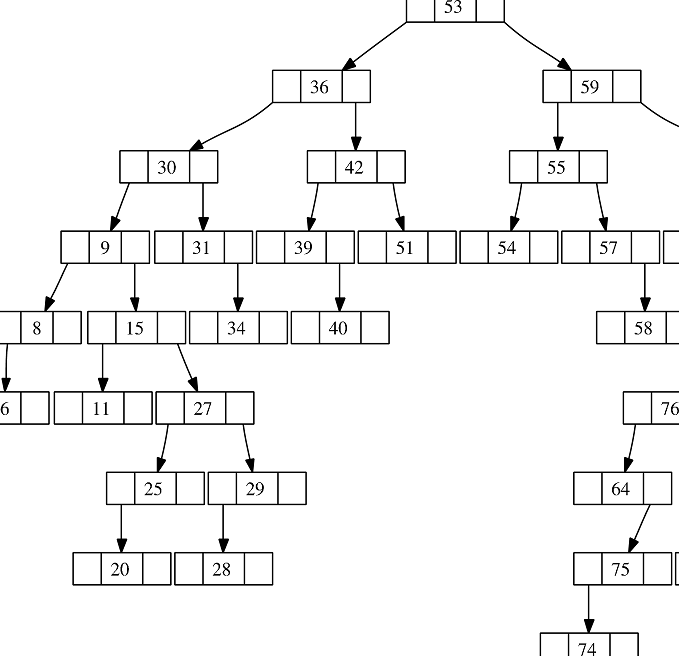
\includegraphics[width=0.8\linewidth]{images/figura_1}
   \caption{Ejemplo de figura}
   \label{tab:intro}
\end{figure}

%%%%%%%%%%%%%%%%%%%%%%%%%%%%%%%%%%%%%%%%%%%%%%%%%%%%%%%%%%%%%%%%%%%%%%%%%%%%%%%
\newpage{\pagestyle{empty}}
\thispagestyle{empty}

\chapter{\LARGE ULL-Prodef}
\label{chapter:prodef}

Prodef es una herramienta desarrollada inicialmente por Andrés Calimero en su TFG. Los repositorios de Prodef están alojados actualmente en la organzación \emph{PAL-ULL} pero se quiere tenerlos también en una organización de GitHub llamada \emph{ULL-prodef}. En este primer apartado se tratará de cumplir tres principales objetivos:

\begin{itemize}
    \item Familiarizarse con Prodef.
    \item Aprender y listar las herramientas necesarias para trabajar en Prodef.
    \item Migrar los repositorios de Prodef a la nueva organización: \textbf{ULL-prodef}
\end{itemize}

Para migrar a la nueva organización se han tenido que adquirir conocimientos sobre GitHub Actions y \href{https://github.com/semantic-release/semantic-release}{semantic release} principalmente

\bigskip
Con el objetivo de facilitar el trabajo a futuros colaboradores, se han creado dos ficheros:
\begin{itemize}
    \item \href{https://github.com/ULL-prodef/prodef/blob/master/INSTALLATION-GUIDE.md}{ProdefInstallationGuide}: Describe los pasos a seguir para instalar Prodef y ejecutar el problema de la mochila
    \item DeveloperToolsList: Lista y explica brevemente las herramientas que se utilizan para el desarrollo de Prodef, además de indicar enlaces para buscar más información
\end{itemize}
\textbf{TODO:} Poner enlaces a los ficheros o poner la información visible de alguna manera

\section{Instalar Prodef y ejecutar un ejemplo}
La primera toma de contacto ha sido instalar prodef y ejecutar el problema de la mochila utilizando únicamente la línea de comandos. Para ello se ha tenido que:
\begin{enumerate}
  \item Clonar el meta repositorio de Prodef: \url{https://github.com/ULL-prodef/prodef.git}
  \item Instalar el meta repositorio y, utilizando meta y los scripts presentes en el package.json, instalar, compilar, y enlazar los subrepositorios haciendo uso de meta (Para ello se debe descargar java, y crear ficheros \textbf{.npmrc} en la raíz de cada repositorio con un token personal de github adecuado).
  \item Poner en marcha un servidor ejecutando la tarea \textbf{npm start} del repositorio \textbf{prodef-solver-jmetal}
  \item Utilizando la herramienta \href{https://curl.se/}{curl} para ejecutar el \href{https://github.com/PAL-ULL/tfg-andres-calimero-prodef-common/blob/master/src/examples/problems/knapsack.json}{problema de la mochila} utilizando una petición http POST. Para obtener el resultado posteriormente realizamos una petición GET
  
\end{enumerate}
\begin{figure}[htb]
   \centering
   
\includegraphics[width=0.5\linewidth]{images/by-nd_88x31}
   \caption{Otra figura}
   \label{fig:intro}
\end{figure}

\section{Listado de herramientas y tecnologías}
Se ha realizado un listado de herramientas utilizadas para el desarrollo y uso de Prodef.
\begin{itemize}
    \item Herramientas para trabajar con Prodef
    \begin{itemize}
        \item \href{https://github.com/mateodelnorte/meta}{meta}
        \item \href{https://www.npmjs.com/package/rollup-plugin-typescript2}{rollup}
        \item \href{https://www.npmjs.com/package/koa}{koa}
        \item \href{https://juanda.gitbooks.io/webapps/content/api/arquitectura-api-rest.html}{API REST}
        \item \href{https://medium.com/dailyjs/how-to-use-npm-link-7375b6219557}{npm link}
        \item \href{https://www.npmjs.com/package/antlr4ts}{antlr4ts}
    \end{itemize}
    \item Herramientas de estilo
    \begin{itemize}
        \item \href{https://github.com/commitizen/cz-cli}{commitizen}
        \item \href{https://www.npmjs.com/package/@commitlint/cli}{commitlint}
        \item \href{https://www.npmjs.com/package/semantic-release}{semantic-release}
    \end{itemize}
\end{itemize}

\textbf{TODO:} Faltan bastantes herramientas por añadir, las iré introduciendo a medida que la investigue.

%%%%%%%%%%%%%%%%%%%%%%%%%%%%%%%%%%%%%%%%%%%%%%%%%%%%%%%%%%%%%%%%%%%%%%%%%%%%%%%
\newpage{\pagestyle{empty}}
\thispagestyle{empty}

\chapter{\LARGE Título del Capítulo 3}
\label{chapter:tres}

Los capítulos intermedios servirán para cubrir los siguientes aspectos: antecedentes, problemática o estado del arte, objetivos, fases y desarrollo del proyecto.

\bigskip
Bla, Bla, Bla, .....

\section{Primera sección de este capítulo}
\section{Segundo apartado de este capítulo}
\section{Tercer apartado de este capítulo}

%%%%%%%%%%%%%%%%%%%%%%%%%%%%%%%%%%%%%%%%%%%%%%%%%%%%%%%%%
\newpage{\pagestyle{empty}}
\thispagestyle{empty}

\chapter{\LARGE Título del Capítulo 4}
\label{chapter:cuatro}

Los capítulos intermedios servirán para cubrir los siguientes aspectos: antecedentes, problemática o estado del arte, objetivos, fases y desarrollo del proyecto.

\bigskip
El capítulo 1 se describió bla, bla, bla …

%%%%%%%%%%%%%%%%%%%%%%%%%%%%%%%%%%%%%%%%%%%%%%%%%%%%%%%%%
\newpage{\pagestyle{empty}}
\thispagestyle{empty}

\chapter{\LARGE Conclusiones y líneas futuras}
\label{chapter:Resultados}

Este capítulo es obligatorio. Toda memoria de Trabajo de Fin de Grado debe incluir unas conclusiones y unas líneas de trabajo futuro 

%%%%%%%%%%%%%%%%%%%%%%%%%%%%%%%%%%%%%%%%%%%%%%%%%%%%%%%%%
\newpage{\pagestyle{empty}}
\thispagestyle{empty}

\chapter{\LARGE Summary and Conclusions}
\label{chapter:Conclusiones}

This chapter is compulsory. The memory should include an extended summary and conclusions in english. 

%%%%%%%%%%%%%%%%%%%%%%%%%%%%%%%%%%%%%%%%%%%%%%%%%%%%%%%%%
\newpage{\pagestyle{empty}}
\thispagestyle{empty}

\chapter{\LARGE Presupuesto}
\label{chapter:presupuesto}

Este capítulo es obligatorio. Toda memoria de Trabajo de Fin de Grado debe incluir un presupuesto.

\section{Sección Uno}

\begin{center}
\begin{tabu} to 0.8\textwidth { | X[l] | X[l] | }
 \hline
 \multicolumn{1}{|c|}{\bf Tipos} & \multicolumn{1}{|c|}{\bf Descripción} \\
 \hline
 AAAA  & BBBB \\
 \hline
 CCCC  & DDDD \\
 \hline
 EEEE  & FFFF \\
 \hline
 GGGG  & HHHH \\
 \hline
\end{tabu}
\end{center}

\begin{table}[htb]
   \centering
   \caption{Resumen de tipos}
   \label{tab:presupuesto}
\end{table}

%%%%%%%%%%%%%%%%%%%%%%%%%%%%%%%%%%%%%%%%%%%%%%%%%%%%%%%%%
\newpage{\pagestyle{empty}\cleardoublepage}
\thispagestyle{empty}

\begin{appendix}

\chapter{\LARGE Título del Apéndice 1}
\label{appendix:1}
\section{Algoritmo XXX}
\label{Apendice1:XXX}

\begin{center}
\begin{footnotesize}
\begin{verbatim}

/***********************************************************************************
*
* Fichero .h
*
***********************************************************************************
*
* AUTORES
*   
*
* FECHA
*   
*
* DESCRIPCION
*   
*
************************************************************************************/

\end{verbatim}
\end{footnotesize}
\end{center}

\section{Algoritmo YYY}
\label{Apendice1:YYY}

\begin{center}
\begin{footnotesize}
\begin{verbatim}


/***********************************************************************************
 *
 * Fichero .h
 *
 ***********************************************************************************
 *
 * AUTORES
 *
 * FECHA
 *
 * DESCRIPCION
 *
 *
 ************************************************************************************/
 
\end{verbatim}
\end{footnotesize}
\end{center}

\section{Algoritmo ZZZ}
\label{Apendice1:ZZZ}

\begin{center}
\begin{footnotesize}
\begin{verbatim}


/***********************************************************************************
 *
 * Fichero .h
 *
 ***********************************************************************************
 *
 * AUTORES
 *
 * FECHA
 *
 * DESCRIPCION
 *
 *
 ************************************************************************************/
 
\end{verbatim}
\end{footnotesize}
\end{center}



\chapter{\LARGE Título del Apéndice 2}
\label{appendix:2}
\section{Otro apéndice: Sección 1}
texto

\section{Otro apéndice: Sección 2}
texto

\end{appendix}

%%%%%%%%%%%%%%%%%%%%%%%%%%%%%%%%%%%%%%%%%%%%%%%%%%%%%%%%%%
\begin{thebibliography}{X}
% Aquí figurará la bibliografía
\end{thebibliography}
%%%%%%%%%%%%%%%%%%%%%%%%%%%%%%%%%%%%%%%%%%%%%%%%%%%%%%%%%%

\end{document}

